\documentclass[tikz]{standalone}
\begin{document}
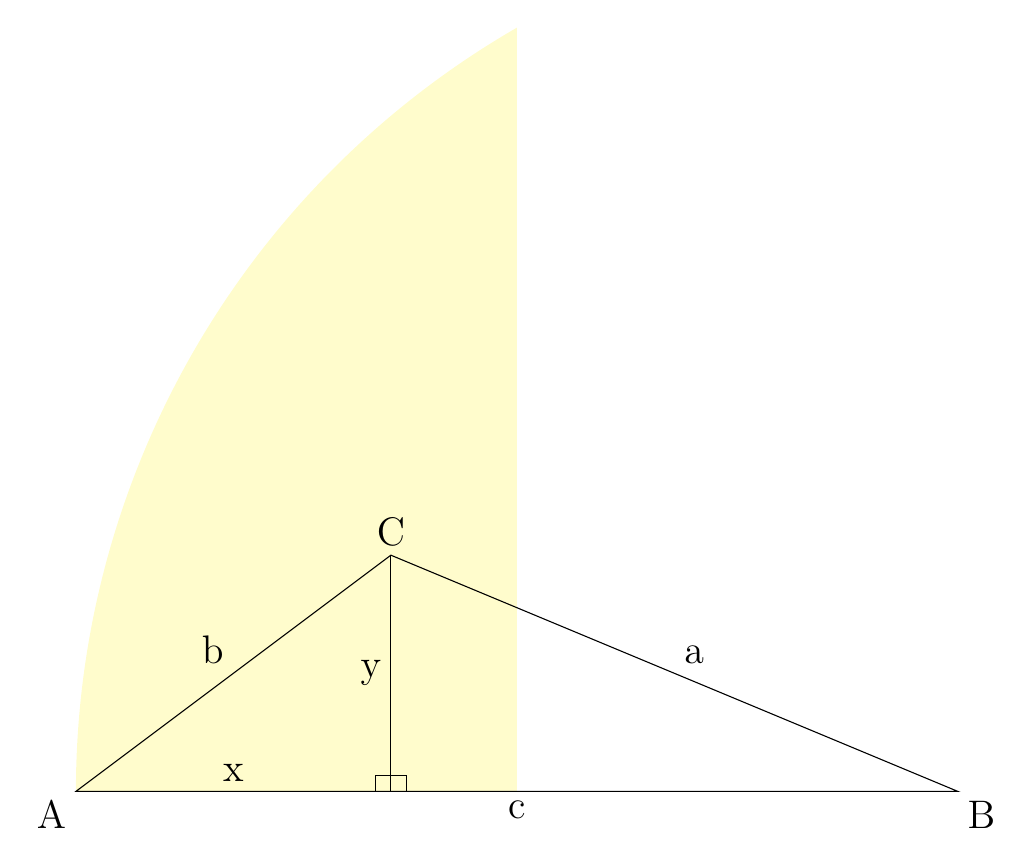
\begin{tikzpicture}
\begin{scope}[scale=0.2]
\fill[yellow!20!white] (28,0) -- (0,0) arc (180:120:56) -- cycle;
%\draw (0,0) arc (180:120:56); \draw (56,0) arc (0:60:56); 
\end{scope}
\begin{scope}[scale=0.2]
\draw (0,0) -- (56,0) -- (20,15) -- cycle;
\draw (20,15) -- (20,0);
\draw (19,0) -- (19,1) -- (21,1) -- (21,0);
\end{scope}
\begin{scope}[scale=0.2, font=\Large]
\draw (0,0) [below left] node{A};\draw (56,0) [below right] node{B};\draw (20,15) [above] node{C};
\draw (38,7.5) [above right] node{a};\draw (10,7.5) [above left] node{b};\draw (28,0) [below] node{c};
\draw (10,0) [above] node{x};\draw (20,7.5) [left] node{y};
\end{scope}
\end{tikzpicture}
\end{document}
